\section{Introducción}

En este entregable se realiza el diseño y análisis de un circuito multiplicador de tensión basado en el Duplicador de Greinacher.
Este circuito, el cual se puede ver en la figura \ref{fig_intro}, se basa en el principio del rectificador de medio puente.

El condensador $C1$ se carga para tensiones de entrada desde $-\hat{V}$ hasta $+\hat{V}$ ($\frac{dV}{dt}$ positivo) y
se descarga a través del diodo $D2$ durante las variaciones de tensión de entrada $\frac{dV}{dt}$ negativas, cargando así el condensador
$C2$. Este proceso se repite durante varios ciclos, hasta llegar a un punto en el que el condensador $C1$ quede cargado a la tensión de pico de la 
senoidal de entrada y el condensador $C2$ al doble de la tensión de pico de entrada. Esto se produce puesto que,
en los ciclos de tensión de entrada negativa, la tensión soportada por el condensador $C2$ es la del condensador $C1$ sumada a la tensión de la fuente.

\begin{figure}[H]
    \centering
    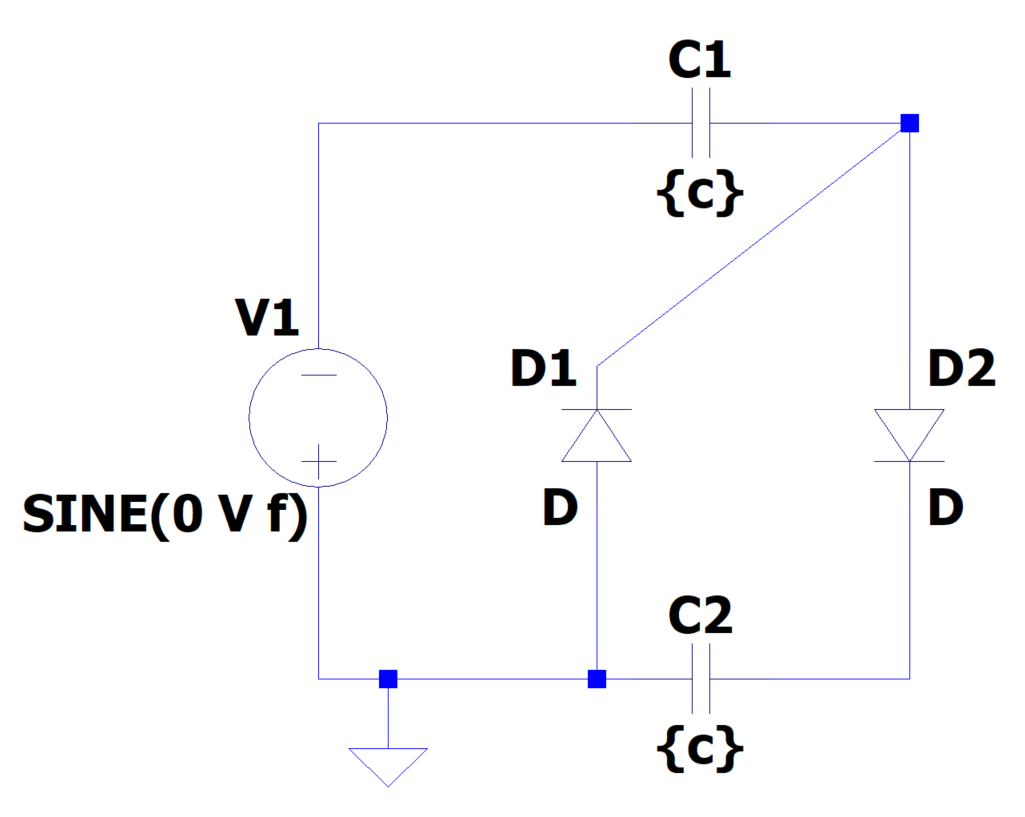
\includegraphics[width=0.6\textwidth]{Imagenes_alvaro/fig_intro.png}
    \caption{Multiplicador de Greinacher de 1 etapa}
    \label{fig_intro}
\end{figure}

Además, cabe destacar que este circuito es escalable, permitiendo de manera teórica obtener tensiones de salida infinitas a partir de fuentes de tensión
oscilatorias de bajo voltaje.

\section{Objetivos}

El principal objetivo de este trabajo es conseguir diseñar un Multiplicador de Greinacher que permita obtener una tensión de salida específica.
Además, debe ser capaz de proveer cierta cantidad de corriente de salida sin que se produzca una caída significativa de la tensión, de manera que será
necesario dimensionar correctamente la capacidad de los condensadores. Por otra parte, el circuito debe ser capaz de funcionar en un rango de frecuencia definido
y para tensiones de entrada senoidales y cuadradas. También será necesario diseñar un circuito que permita medir la tensión de salida a partir de un multímetro.
Todos los requisitos se definen de manera específica en la sección \ref{requisitos}

\section{Establecimiento de requerimientos} \label{requisitos}